\documentclass[10pt]{article}
\usepackage[margin=0.4in]{geometry}
\usepackage{amsmath}
\usepackage{tikz}
\usetikzlibrary{arrows.meta,positioning,backgrounds,fit,calc}
\pagestyle{empty}

\definecolor{cafeblue}{HTML}{2B6CB0}
\definecolor{cafeteal}{HTML}{2C7A7B}
\definecolor{cafeamber}{HTML}{C05621}
\definecolor{caferred}{HTML}{C53030}
\definecolor{cafeslate}{HTML}{475569}
\definecolor{cafebg}{HTML}{F1F5F9}
\definecolor{cafegrey}{HTML}{94A3B8}

\newcommand{\ubt}[3]{\textcolor{#1}{\underbrace{#2}_{\text{\scriptsize #3}}}}

\begin{document}
\begin{figure}
\centering
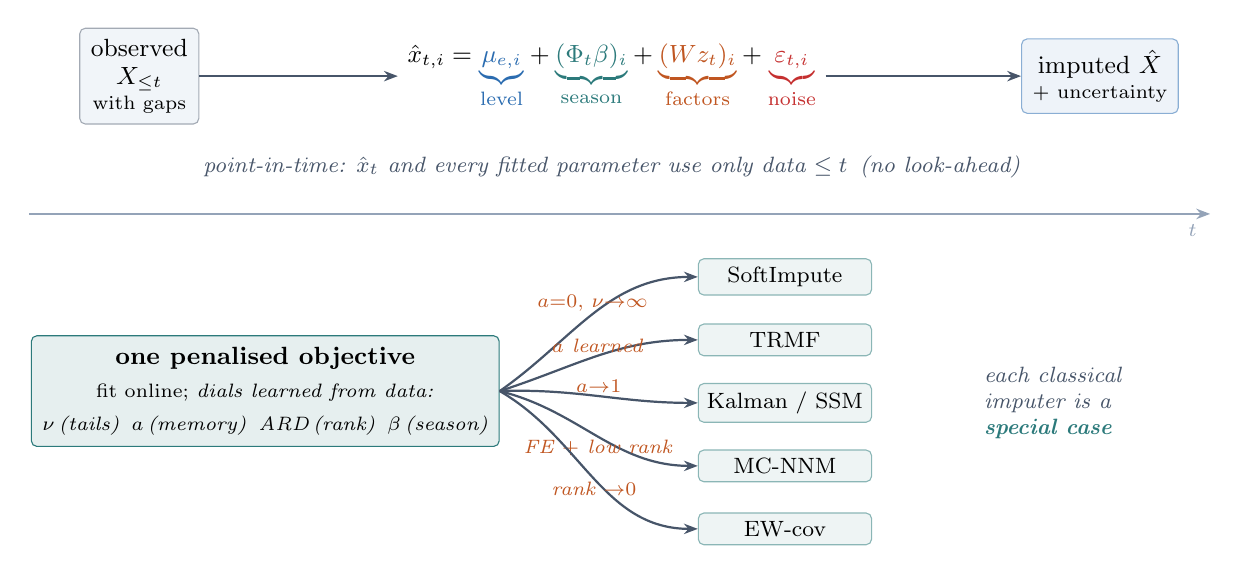
\begin{tikzpicture}[
  font=\small,
  term/.style={rounded corners=2pt, draw=cafeslate!50, fill=white, inner sep=4pt,
               minimum height=9mm, align=center},
  lf/.style={-{Stealth[length=5pt]}, cafeslate, line width=0.8pt},
  leaf/.style={rounded corners=2pt, draw=cafeteal!55, fill=cafeteal!8, inner sep=3pt,
               font=\footnotesize, align=center, minimum width=22mm},
  dial/.style={font=\scriptsize\itshape, cafeamber, inner sep=1pt},
]

% ===== ROW 1 : the causal additive decomposition =====
\node[term, fill=cafebg] (X) at (0,0) {observed\\[-1pt]$X_{\le t}$\\[-2pt]\scriptsize with gaps};
\node[term, draw=cafeblue!55, fill=cafeblue!8] (fill) at (12.2,0)
   {imputed $\hat{X}$\\[-2pt]\scriptsize $+$ uncertainty};
\node (eq) at (6.0,0) {$\displaystyle \hat{x}_{t,i}=
   \ubt{cafeblue}{\mu_{e,i}}{level}+
   \ubt{cafeteal}{(\Phi_t\beta)_i}{season}+
   \ubt{cafeamber}{(Wz_t)_i}{factors}+
   \ubt{caferred}{\varepsilon_{t,i}}{noise}$};
\draw[lf] (X.east) -- (eq.west);
\draw[lf] (eq.east) -- (fill.west);

% causal strip just under row 1
\node[font=\footnotesize\itshape, cafeslate] (cap) at (6.0,-1.15)
   {point-in-time: $\hat{x}_t$ and every fitted parameter use only data $\le t$\, (no look-ahead)};
\draw[-{Stealth[length=5pt]}, cafegrey, line width=1pt]
   (-1.4,-1.75) -- node[below, font=\scriptsize, pos=0.985]{$t$} (13.6,-1.75);

% ===== ROW 2 : one objective -> classical methods as special cases =====
\node[term, fill=cafeteal!12, draw=cafeteal, align=center, minimum width=34mm] (obj) at (1.6,-4.0)
   {\textbf{one penalised objective}\\[1pt]
    {\scriptsize fit online; \emph{dials learned from data:}}\\[1pt]
    {\scriptsize\itshape $\nu$\,(tails)\, $a$\,(memory)\, ARD\,(rank)\, $\beta$\,(season)}};

\node[leaf] (l1) at (8.2,-2.55) {SoftImpute};
\node[leaf] (l2) at (8.2,-3.35) {TRMF};
\node[leaf] (l3) at (8.2,-4.15) {Kalman / SSM};
\node[leaf] (l4) at (8.2,-4.95) {MC-NNM};
\node[leaf] (l5) at (8.2,-5.75) {EW-cov};

\draw[lf] (obj.east) to[out=35,in=180]  node[dial,above,pos=0.5]{$a{=}0,\,\nu{\to}\infty$} (l1.west);
\draw[lf] (obj.east) to[out=18,in=180]  node[dial,above,pos=0.5]{$a$ learned} (l2.west);
\draw[lf] (obj.east) to[out=2,in=180]   node[dial,above,pos=0.5]{$a{\to}1$} (l3.west);
\draw[lf] (obj.east) to[out=-14,in=180] node[dial,below,pos=0.5]{FE $+$ low rank} (l4.west);
\draw[lf] (obj.east) to[out=-30,in=180] node[dial,below,pos=0.5]{rank ${\to}0$} (l5.west);

\node[font=\footnotesize\itshape, cafeslate, align=left] at (11.6,-4.15)
   {each classical\\ imputer is a\\ \textbf{\textcolor{cafeteal}{special case}}};

\end{tikzpicture}
\end{figure}
\end{document}
